\documentclass[10pt,a4paper,oneside]{article}

\usepackage[swedish]{babel}
\usepackage[utf8]{inputenc}
\usepackage[T1]{fontenc}
\usepackage{graphicx}
\usepackage{color}
\usepackage{url}
\usepackage{hyperref}
\usepackage[nomarkers]{endfloat}

\renewcommand{\efloatseparator}{\mbox{}} % allows tables to share a page
 
\title{XXX}
\author{Erica Eriksson, Johanna Sörbom, Malin Torestam}
\date{\today}

\begin{document}

\maketitle
\newpage

\section{Sammanfattning}
I denna rapport presenteras en affärsmodell för XXX. Detta är en nätbaserad tjänst som främjar försäljning av närproducerade produkter. XXX vill förenkla för småskaliga producenter i Stockholmsområdet att konkurrera med importerade varor från butiker och nå ut till fler miljömedvetna kunder. Detta är en tjänst som ligger i tiden och fyller ett växande behov i ett samhälle där miljö- och klimattänk blir allt vanligare. I denna rapport diskuteras affärsmodellens hållbarhet i olika framtidsscenarion och alternativa utvecklingar av modellen för att klara av att konkurrera på dagens marknad. I den riktning samhället är på väg mot förväntas denna affärside ha en bra chans att växa sig stark. Dock finns det alltid osäkerheter och svagheter med affärsmodeller som kommer att diskuteras i detalj i denna rapport. 
\newpage

\tableofcontents
\newpage

\section{Introduktion}
\newpage

\section{Bakgrund}
\newpage

\section{Metod}
\newpage

\section{Beskrivning av tjänsten}
\subsection{Vad erbjuder vi för tjänst?}
\subsection{Hur blir man medlem?}
\subsection{Vad krävs för att bli medlem?}
\subsection{Hur ska hemsidan och appen utformas?}
\subsection{Kvalitetskontroll}
\subsection{Förpackning av varor}
\subsection{Order och leverans}
\subsection{Framtida expansionsmöjligheter för tjänsten }
\newpage

\section{Koppling till energisystemet}
\newpage

\section{Canvas modellen}
\subsection{Värdeerbjudande}
\subsection{Kundsegment}
\subsection{Kanaler}
\subsection{Kundrelation}
\subsection{Intäktsström}
\subsection{Nyckelresurser}
\subsection{Nyckelaktiviteter}
\subsection{Nyckelpartners}
\subsection{Kostnadsstruktur}
\newpage

\section{Marknadsundersökning}
\newpage

\section{Ekonomisk budget}
\newpage

\section{Konkurrenter}
\newpage

\section{Analyser}
\subsection{Val av affärsmodell}
\subsection{Scenarioanalys  - yttre faktorer}
\subsection{SWOT- analys}
\newpage

\section{Diskussion}
\newpage

\section{Slutsats}
\newpage

\bibliographystyle{amsplain}
\bibliography{litterature}
\newpage

\begin{figure}
	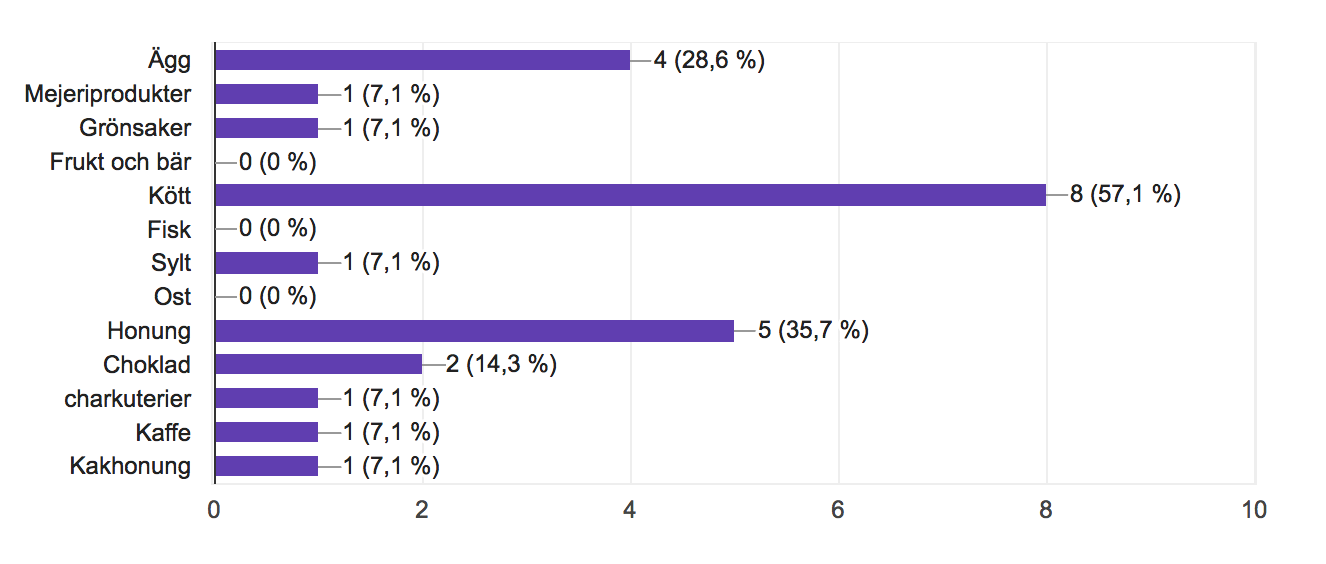
\includegraphics[scale=0.6]{1.png}
	\caption{Vad s\"aljer du f\"or typ av produkter?}
\end{figure}

\begin{figure}
	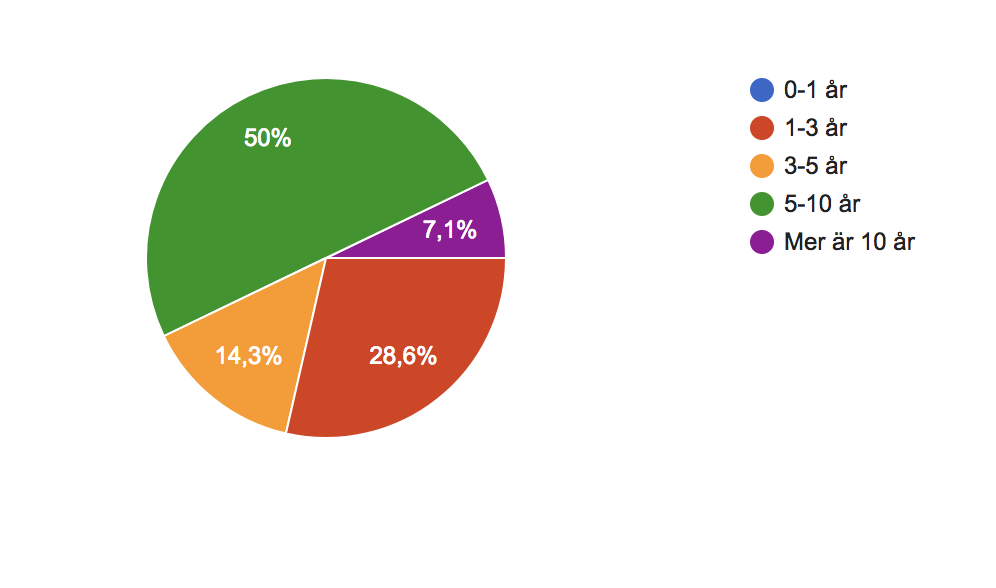
\includegraphics[scale=0.6]{2.png}
	\caption{Hur l\"ange har du s\'alt dessa varor?}
\end{figure}

\begin{figure}
	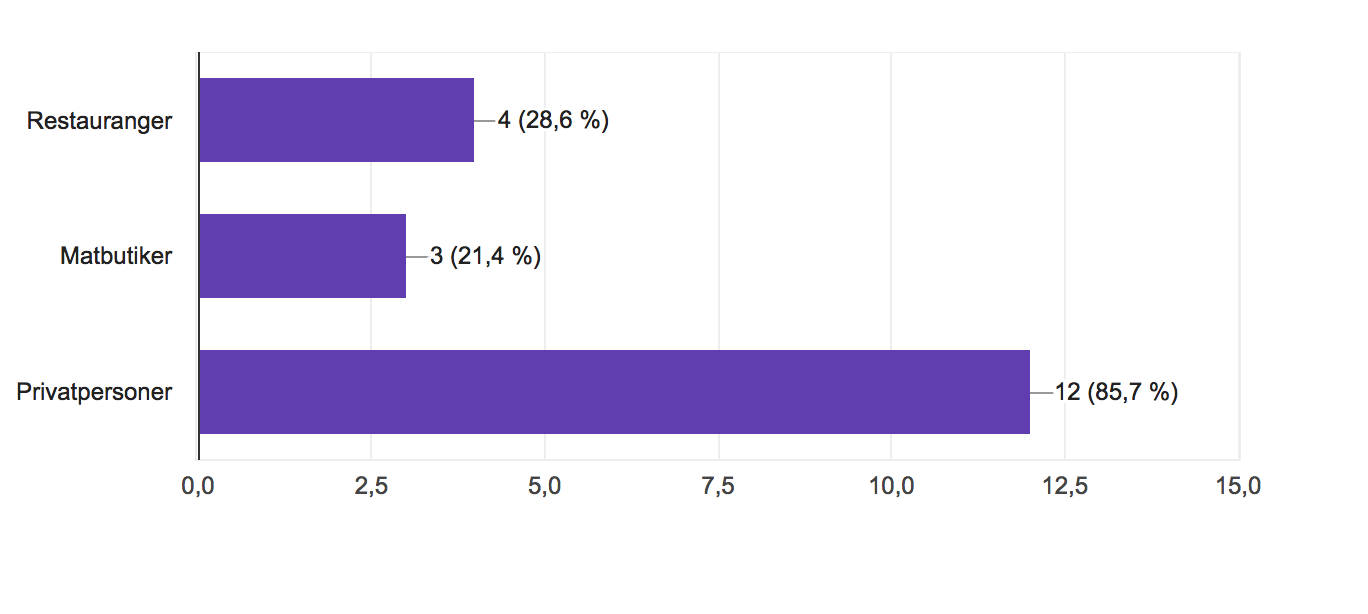
\includegraphics[scale=0.6]{3.png}
	\caption{Vad \"ar din huvudsakliga kundkrets?}
\end{figure}

\begin{figure}
	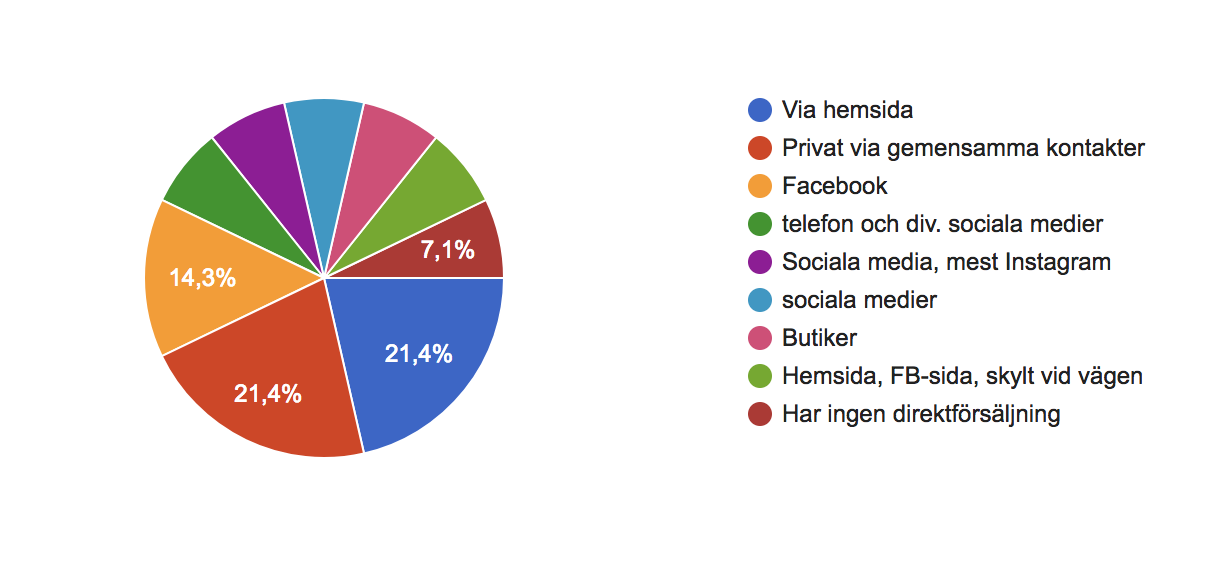
\includegraphics[scale=0.6]{4.png}
	\caption{P\'a vilket s\"att kommer kunder i kontakt med dig idag?}
\end{figure}

\begin{figure}
	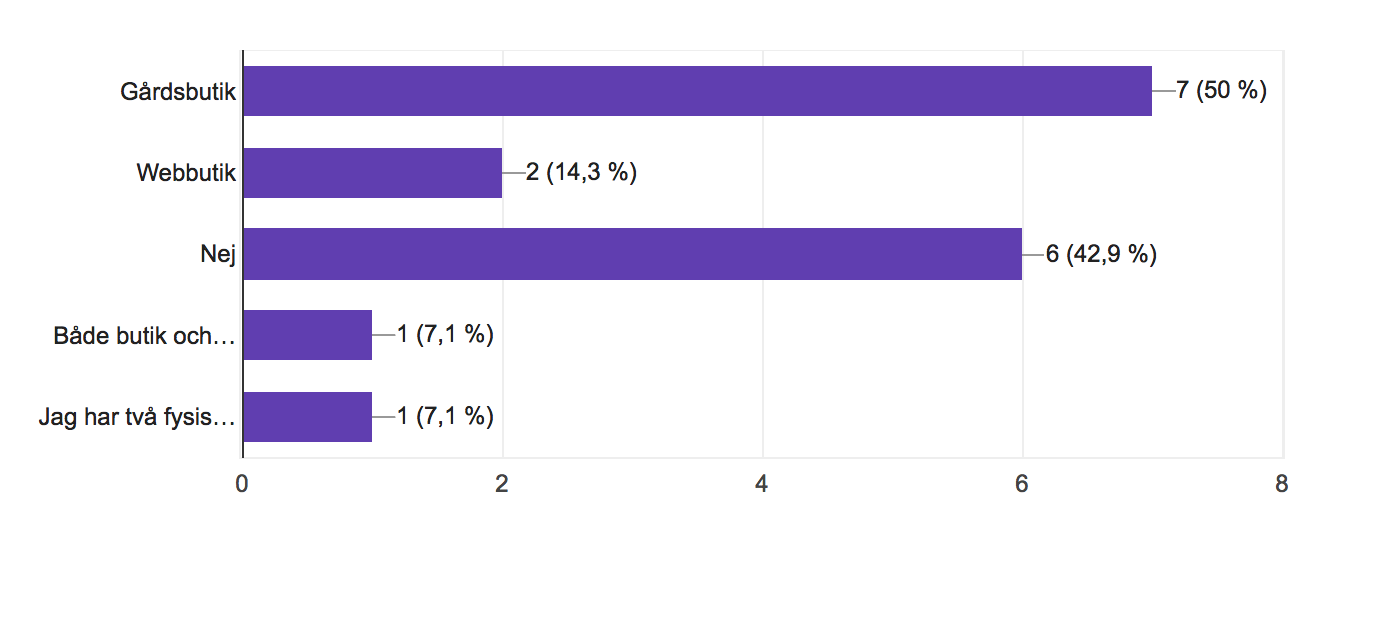
\includegraphics[scale=0.6]{5.png}
	\caption{Har du i dagsl\"aget en g\'ardsbutik eller webbutik?}
\end{figure}

\begin{figure}
	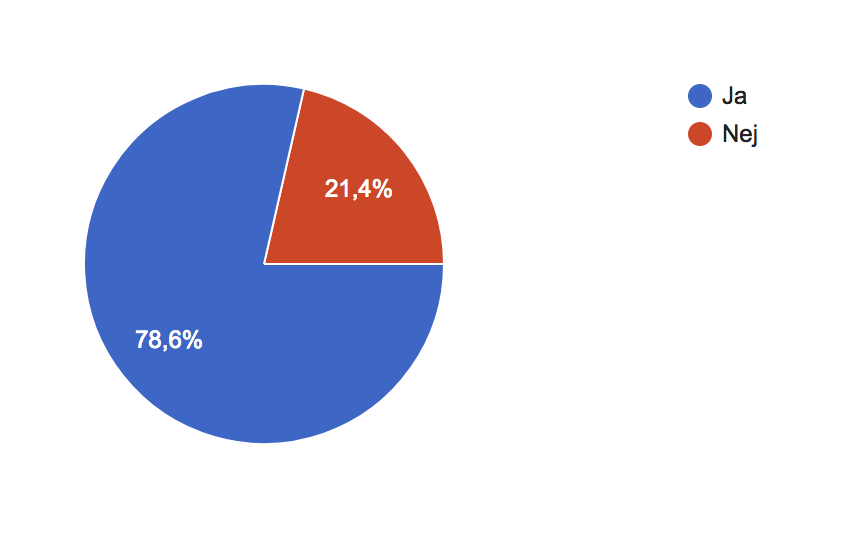
\includegraphics[scale=0.6]{6.png}
	\caption{Skulle du vara intresserad av att n\'a ut till fler privatpersoner?}
\end{figure}

\begin{figure}
	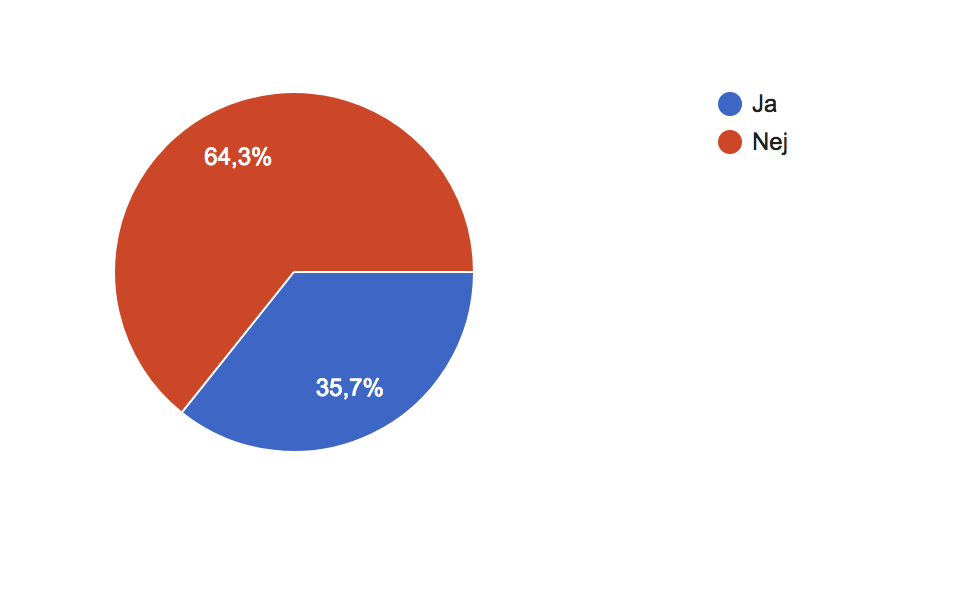
\includegraphics[scale=0.6]{7.png}
	\caption{Tror du att majoriteten av m\"ojliga kunder k\"anner till dig och vad du s\"aljer när de ska k\"opa varor som du kan leverera?}
\end{figure}

\begin{figure}
	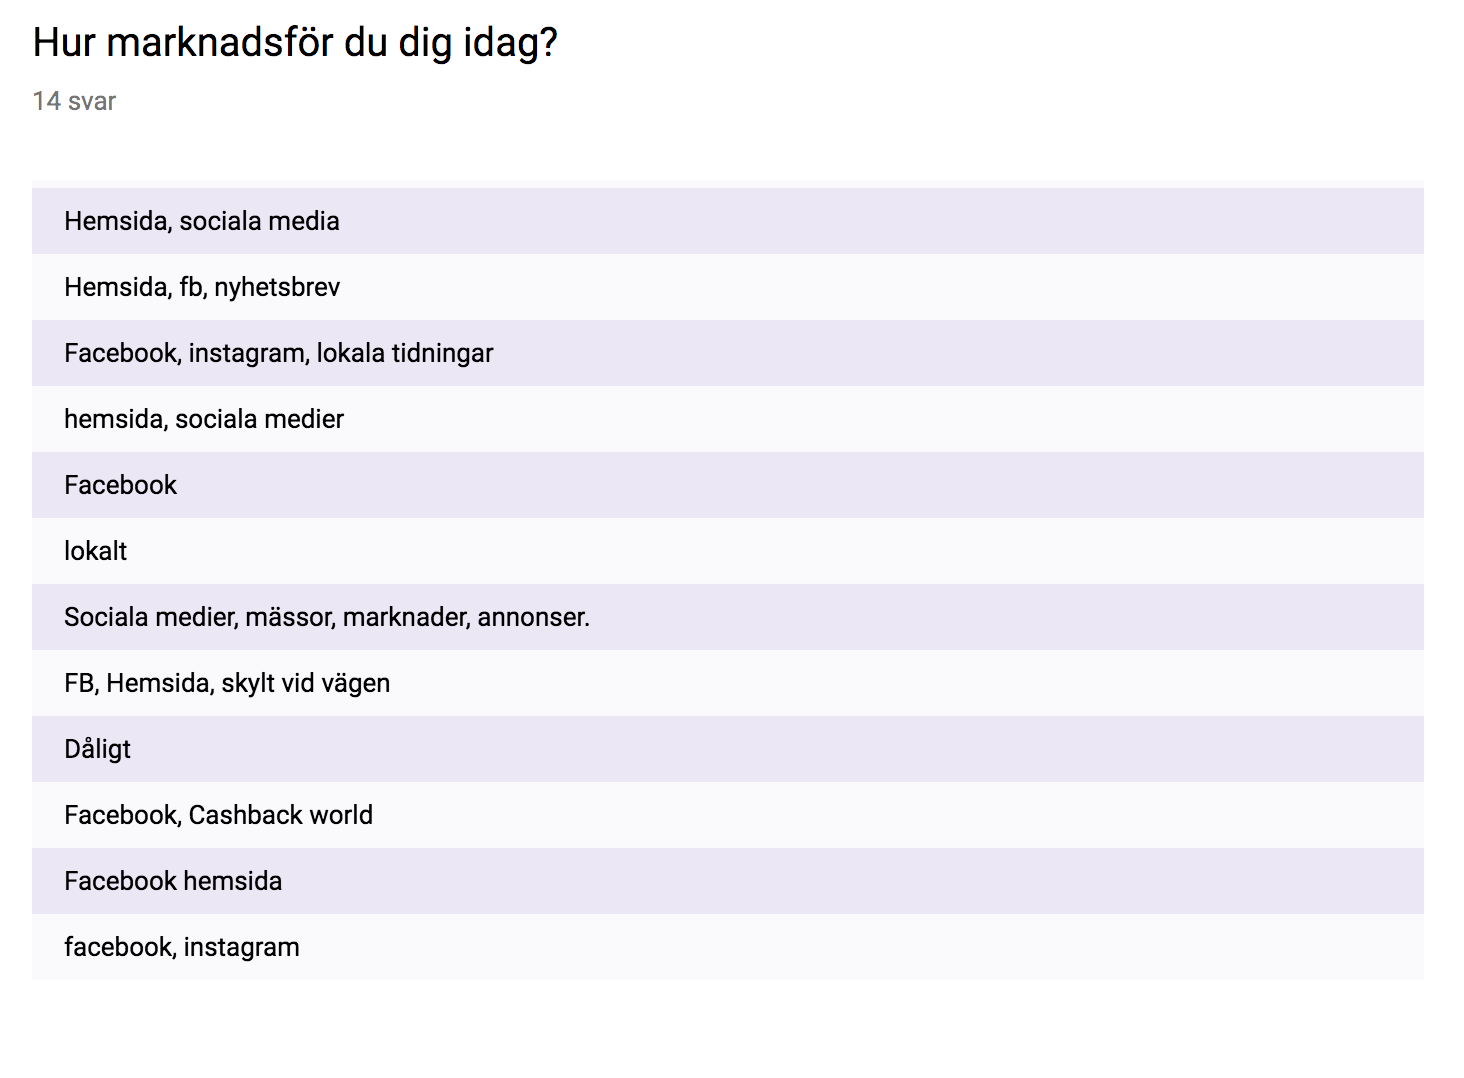
\includegraphics[scale=0.6]{8.png}
	\caption{Hur marknadsf\"or du dig idag?}
\end{figure}

\begin{figure}
	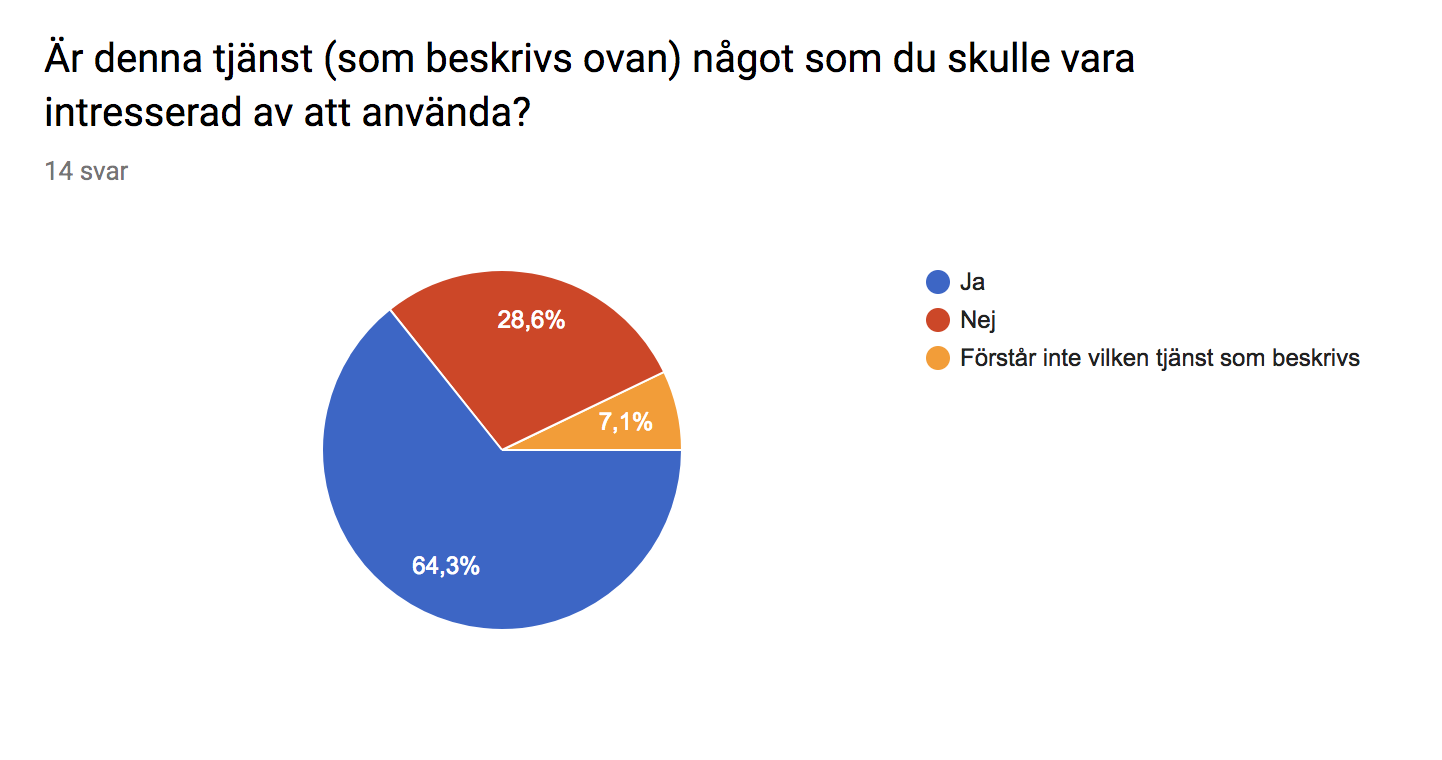
\includegraphics[scale=0.6]{9.png}
	\caption{Är denna tj\"anst n\'agot som du skulle vara intresserad av att anv\"anda?}
\end{figure}

\begin{figure}
	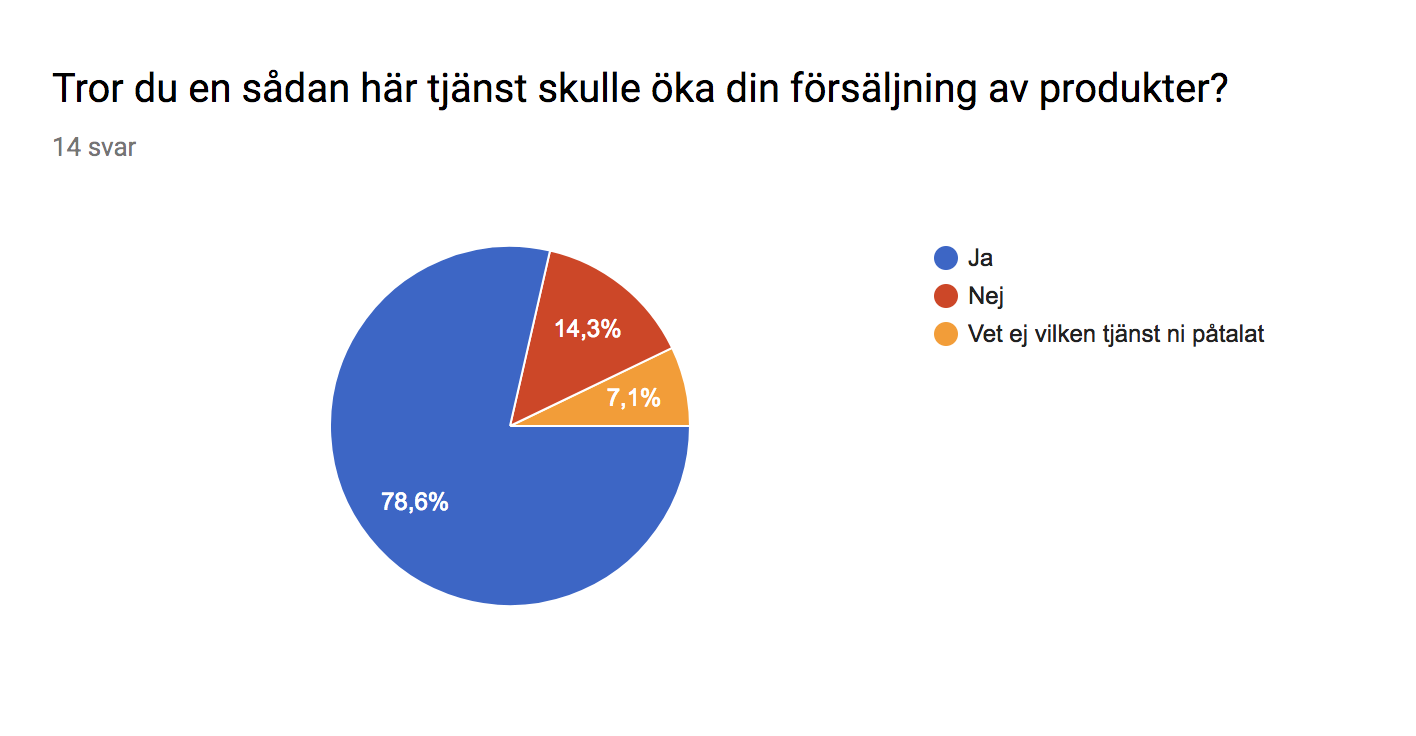
\includegraphics[scale=0.6]{10.png}
	\caption{Tror du att en s\'adan h\"ar tj\"anst skulle \"oka din f\"olrs\"aljning av produkter?}
\end{figure}

\begin{figure}
	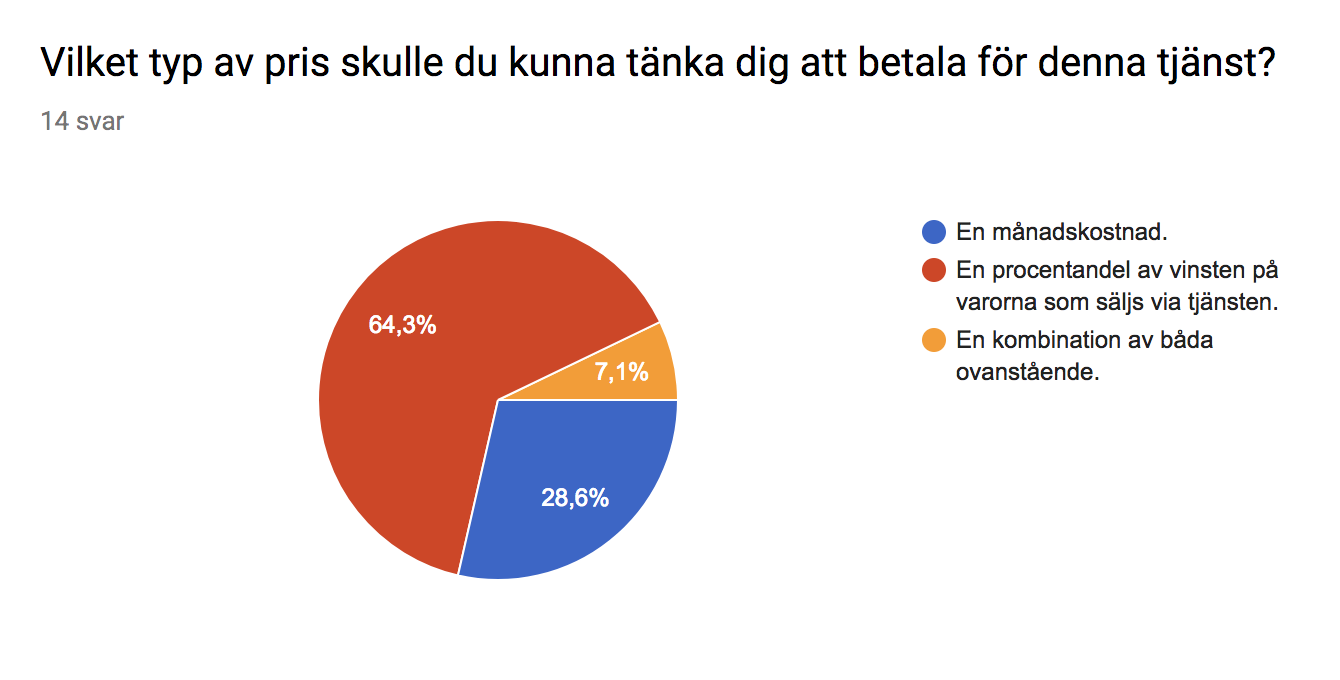
\includegraphics[scale=0.6]{11.png}
	\caption{Vilken typ av pris skulle du kunna t\"anka dig att betala för denna tj\"anst?}
\end{figure}

\begin{figure}
	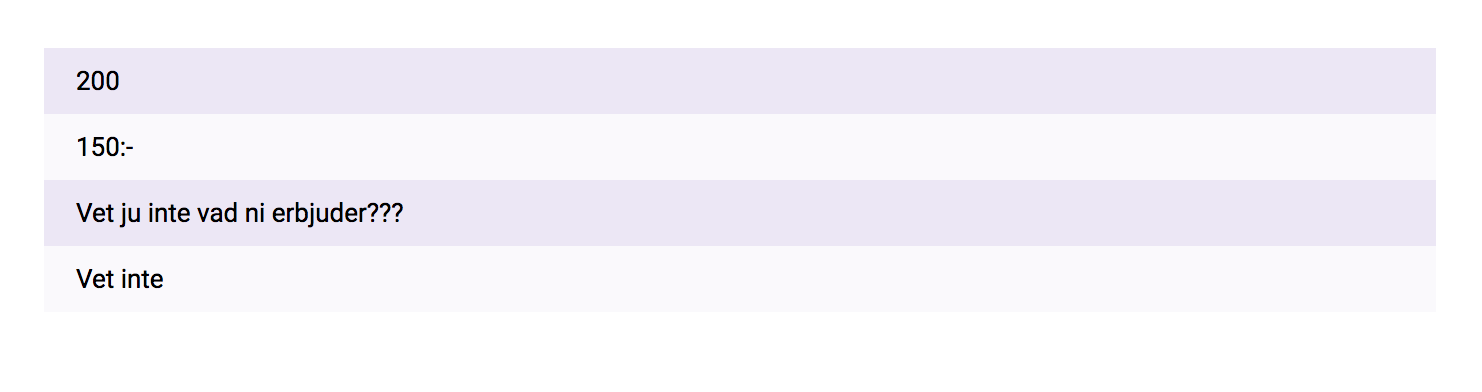
\includegraphics[scale=0.6]{12.png}
	\caption{Om en m\'anadskostnad, hur mycket?}
\end{figure}

\begin{figure}
	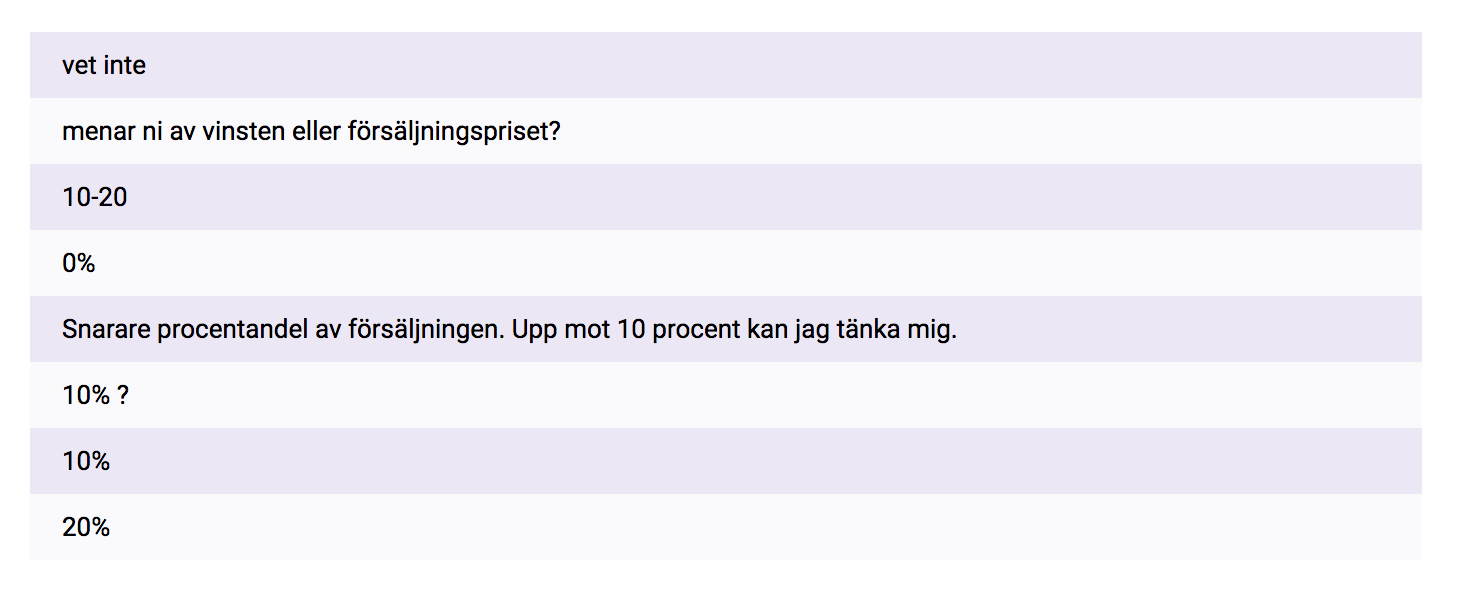
\includegraphics[scale=0.6]{13.png}
	\caption{Om en procentandel, hur mycket?}
\end{figure}

\begin{figure}
	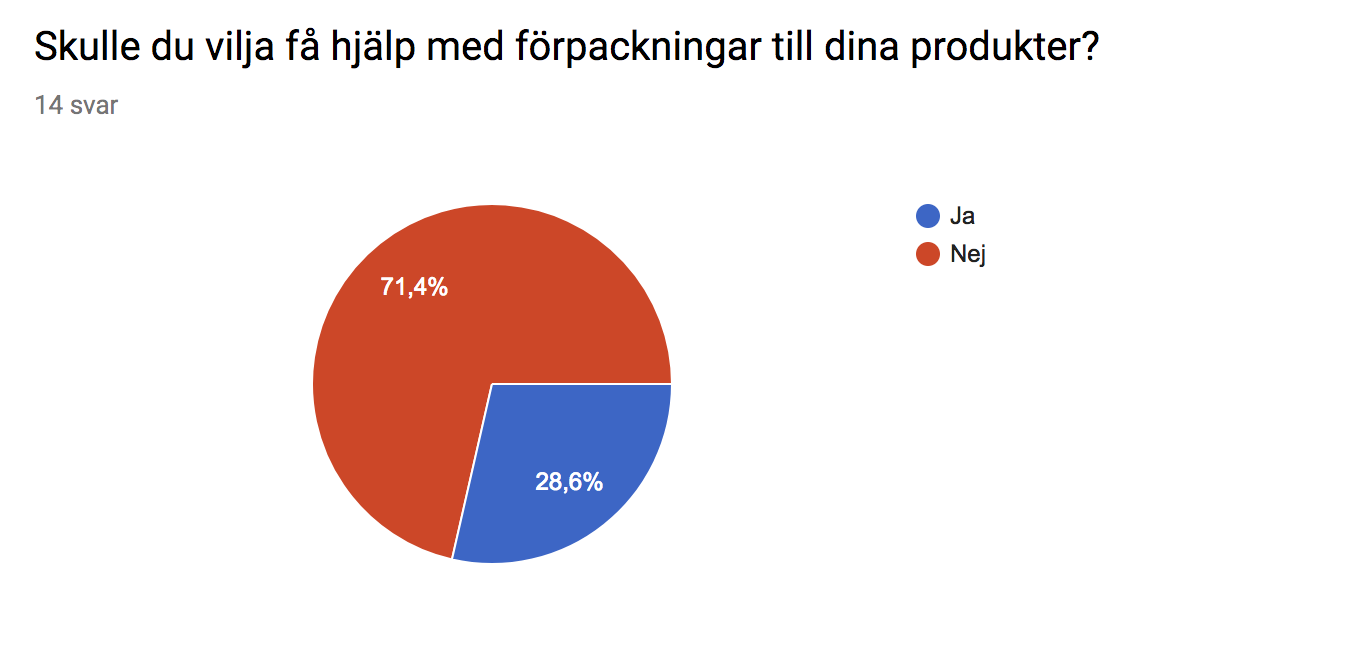
\includegraphics[scale=0.6]{14.png}
	\caption{Skulle du vilja f\'a hj\"alp med f\"orpackningar till dina produkter?}
\end{figure}

\end{document}